

% ****** Start of file aipsamp.tex ****m*
%
%   This file is part of the AIP files in the AIP distribution for REVTeX 4.
%   Version 4.1 of REVTeX, October 2009
%
%   Copyright (c) 2009 American Institute of Physics.
%
%   See the AIP README file for restrictions and more information.
%
% TeX'ing this file requires that you have AMS-LaTeX 2.0 installed
% as well as the rest of the prerequisites for REVTeX 4.1
% 
% It also requires running BibTeX. The commands are as follows:
%
%  1)  latex  aipsamp
%  2)  bibtex aipsamp
%  3)  latex  aipsamp
%  4)  latex  aipsamp
%
% Use this file as a source of example code for your aip document.
% Use the file aiptemplate.tex as a template for your document.
\documentclass[%
 aps, pra,
% jmp,
% bmf,
% sd,
% rsi,
 amsmath,amssymb,
%preprint,%
 reprint,%
%author-year,%
%author-numerical,%
% Conference Proceedings
superscriptaddress
]{revtex4-2}

\usepackage{graphicx}% Include figure files
%\usepackage{dcolumn}% Align table columns on decimal point
\usepackage{bm}% bold math
\usepackage{fixme}
%\usepackage[mathlines]{lineno}% Enable numbering of text and display math
%\linenumbers\relax % Commence numbering lines
\usepackage{hyperref}
\usepackage{kbordermatrix}% http://www.hss.caltech.edu/~kcb/TeX/kbordermatrix.sty
\usepackage[utf8]{inputenc}
\usepackage[T1]{fontenc}
\usepackage{mathptmx}
\usepackage{lipsum}
\usepackage{amsmath}
\usepackage{physics}
\usepackage{xparse}
\usepackage{bbm}
\usepackage{xcolor}
\usepackage{url}


%\usepackage{multirow}
%\usepackage{makecell}
\graphicspath{{Pictures/}}

\renewcommand*{\figureautorefname}{Fig.}
\renewcommand*{\equationautorefname}{Eq.}

\newcommand{\mytitile}{Photon transport and chaos in a Bose-Hubbard chain of superconducting artificial atoms}

\begin{document}
	\preprint{AIP/123-QED}
	
	\title[\mytitile]{\mytitile\\~}
	\author{G.P. Fedorov}
	\email{gleb.fedorov@phystech.edu}
	
	\affiliation{ 
		Russian Quantum Center, Skolkovo village, Russia
	}%
	\affiliation{ 
		Moscow Institute of Physics and Technology, Dolgoprundiy, Russia
	}
	\affiliation{
		National University of Science and Technology MISIS, Moscow, Russia
	}%

	\author{I.A. Rodionov}
	\affiliation{FMN Laboratory, Bauman Moscow 
	State Technical University, Moscow, Russia}
	\affiliation{Dukhov Automatics Research 
	Institute, (VNIIA), Moscow, Russia}

	\author{O.V. Astafiev}
	\affiliation{Skolkovo Institute of Science 
		and Technology, Moscow, Russian Federation}
	\affiliation{ 
		Moscow Institute of Physics and Technology, 
		Dolgoprundiy, Russia
	}
	\affiliation{Physics Department, Royal 
	Holloway, University of London, Egham, Surrey 
	TW20 0EX, United Kingdom}
\affiliation{National Physical Laboratory, Teddington, TW11 0LW, United Kingdom}
%
	
	
	\date{\today}% It is always \today, today,
	%  but any date may be explicitly specified
	
	
	\begin{abstract}
We investigate non-equilibrium steady-state photon transport through a chain of five coupled artificial atoms described by the Bose-Hubbard model. By increasing incident photon flux, we demonstrate a continuous transition from the linear regime described by the classical coupled oscillators model to the quantum regime of photon blockade characterized by suppressed transmission and complex structure of multiphoton resonances. We show excellent agreement of the transmission with the input-output theory for a model with around a hundred basis states. Next, we demonstrate that our architecture allows straightforward and high-contrast visualization of the emergent energy bands via cross-Kerr spectroscopy. Finally, we show how controllable disorder in the system suppresses this non-local photon transmission. We argue that our architecture may be applied for analog simulation of many-body Floquet dynamics with even larger arrays of artificial atoms paving an alternative way to quantum supremacy.
\end{abstract}
	
\maketitle

\section{Introduction}


There has been increased effort over recent years in analog simulation of various models from solid state physics and quantum optics on a chip using superconducting circuits \cite{kjaergaard2019superconducting}. The Bose-Hubbard (B-H) model is now particularly well-covered as it can be directly mapped onto arrays of coupled transmons \cite{orell2019probing}. The first work \cite{hacohen2015cooling} had demonstrated this for a three-site linear lattice, and subsequent experiments were focused either on simulating dynamics with engineered dissipation \cite{ma2019dissipatively}, or studying the many-body localization phase transitions \cite{roushan2017spectroscopic,chiaro2019growth}, or correlated quantum walks \cite{Yan2019, Ye2019}.

Numerous theoretical studies propose a new possible direction: controllable light-matter interaction and Floquet engineering to model periodically-driven Hamiltonians and their non-equilibrium dynamics \cite{Goldman2014, eisert2015quantum, Zippilli2015, kyriienko2018floquet, franca2020simulating}. Particularly, a recent study has shown that this approach may open new ways for quantum supremacy \cite{tangpanitanon2019quantum}.

In this Letter, we present a proof-of-principle device to model non-equilibrium steady-state boson transport through a Bose-Hubbard chain.  Transmission properties of artificial materials composed of qubits attracted theoretical research before \cite{Zagoskin2016, viehmann2013observing, Greenberg2015, Fistul2019, Biella2015}; however, apart from purely academic interest, our experiment shows that continuously driven transmon arrays are currently very simple to design and control, and thus seem to be suitable for supremacy-scale Floquet quantum simulations. \textbf{platform for matrix product states, more about blockade}

The layout of the chip is shown in \autoref{fig:scheme}~(a). Similar to previous experiments, we use a chain of directly coupled Xmon transmons tunable via individual flux lines. The distinctive feature is the large interdigitated capacitors to couple the edge transmons strongly to the input and output waveguides and allow measurement of the microwave transmission through the chain. The individual readout resonators are used only for calibration purposes in our experiment.

In \autoref{fig:scheme}~(b), we show the physical model that is being simulated by the device. The corresponding Hamiltonian including the classical drive in RWA is
\begin{equation}
\begin{aligned}
\hat H/\hbar &= \sum_{i=1}^5 (\omega_i - \omega_d) \hat b^\dag_i \hat b_i + \frac{1}{2} \alpha_i \hat b_i^\dag \hat b_i (\hat b^\dag_i \hat b_i - 1)\\
&+\sum_{i=1}^4 J (\hat b^\dag_{i+1} \hat b_i + \hat b_{i+1} \hat b_i^\dag) \\
&+\frac{\Omega}{2}(\hat b_1^\dag + \hat b_1),
\end{aligned}\label{eq:bose-hubbard}
\end{equation} 
where $\hat b_i$, $\hbar \omega_i$ and $\hbar\alpha_i$ are, respectively, the lowering operator, single-boson energy and the on-site interaction for the $i$\textsuperscript{th} site, $J$ is the inter-site tunneling rate, and $\omega_d$ is the drive frequency.

The dissipation in the system is essential to the dynamics as it mostly comes from the waveguides and is included in the corresponding Liouville equation using Lindbladian superoperators 
\begin{equation}
	\mathcal D[\hat{O}^{(i)}_\alpha] = \hat{O}^{(i)}_\alpha \hat \rho \hat{O}^{(i)\dag}_\alpha - \frac{1}{2}\{\hat{O}^{(i)\dag}_\alpha \hat{O}^{(i)}_\alpha, \hat \rho\},
\end{equation}
where $\hat{O}^{(i)}_\gamma = \sqrt{\gamma_i} \hat b_i$ is the relaxation and $\hat{O}^{(i)}_\phi = \sqrt{\gamma^{(i)}_\phi} \hat b_i^\dag \hat b_i$ is the pure dephasing. $\gamma_1 = \gamma_5 = \Gamma \gg \gamma_i, \gamma_\phi^{(i)}, i=2,3,4$.


\begin{figure}
	\centering
	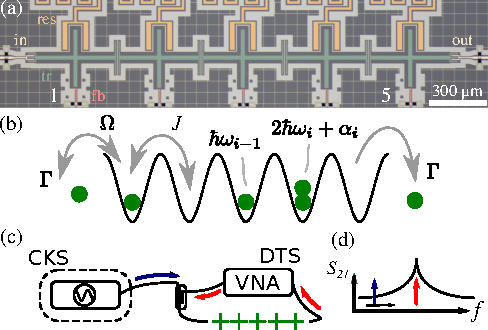
\includegraphics[width=1\linewidth]{Pictures/scheme.pdf}
	\caption{\textbf{(a)} Optical image of the device (false-colored). Input and output waveguides (beige) are strongly coupled to the edge transmons (green), which can be dispersively read out via auxiliary resonators (orange) and tuned via flux lines (red). \textbf{(b)} Interpretation of the device as a B-H lattice with five sites. Bosons are inserted from the left by a drive of strength $\Omega$, and can leak from both sides at rate $\Gamma$. The energy of a localized boson is $\hbar \omega$, and adding another boson to the same site costs $U = \hbar \alpha$. Excitations can tunnel back and forth between sites at rate $J$. \textbf{(c)} Qualitative measurement scheme: the direct transmission (DT) spectroscopy is done using the vector network analyzer which measures the complex transmission $ S_{21} $. The cross-Kerr (C-K) spectroscopy requires an additional microwave source. \textbf{(d)} The C-K spectroscopy is done by sweeping the source frequency (blue arrow) while monitoring the transmission amplitude at some resonance peak via the VNA (red arrow).}
	\label{fig:scheme}
\end{figure}
	

In \autoref{fig:scheme}~(c) we show schematically the experimental setup. We measure the transmission $S_{21}$ through the chain via a vector network analyzer (VNA), and optionally use an additional microwave source to perform the cross-Kerr spectroscopy of the system. Since the microwave signals in our setup are continuous, we are only studying the steady-state properties of the device.

To obtain theoretical predictions for the $S_{21}$ in the steady state, one can use the input-output formalism \cite{yurke1984quantum,gardiner1985input}. Since we irradiate the system coherently, we assume that the input field mode amplitude is related to the classical drive strength $\Omega$ in the driving operator $\hbar \Omega \hat b_1 \cos \omega t$ via $\sqrt{\gamma_1} \langle  \hat b_{in}^\dag \rangle \approx i \Omega/2$, which follows from the quantum Langevin equations when disregarding the noise term. Similarly, the output field operator $\hat b_{out}^\dag \approx \sqrt{\gamma_5} \hat b_5^\dag$. From this, we obtain
\begin{equation}
	S_{21} = \frac{\langle \hat b_{out}^\dag \rangle}{\langle \hat b_{in}^\dag \rangle} = \frac{2\Gamma }{i\Omega} \Tr[\hat \rho_{ss} \hat b_5^\dag],\label{eq:s21}
\end{equation}
where $\hat \rho_{ss}$ is calculated from $\mathcal L \rho_{ss} = 0$. Physically, this expression means that the signal transmission would be possible if the rightmost transmon becomes excited while the leftmost one is subject to radiation. 

However, this apparently non-local excitation of the transmon at the opposite edge of the chain is not a purely quantum-mechanical effect. From the Langevin equations follows that in the limit of zero anharmonicity $\alpha_i = 0$ or, alternatively, $\Omega \ll \Gamma$, the system can be regarded as a chain of classical coupled harmonic oscillators. At the \textit{degeneracy point} when $\omega_i = \omega$, the equivalent classical model nevertheless produces transmission peaks at detunings $\delta = 0,\, \pm J,\, \pm \sqrt{3} J$ from $\omega$, corresponding to the classical normal mode frequencies (see Appendix \ref{sec:app_linear}). In the quantum-mechanical limit, these resonances should remain in the spectrum due to the correspondence principle; however, new lines caused by purely quantum-mechanical processes are expected to appear.

\section{Classical normal modes and quantum eigenstates}

To investigate the differences between the classical and quantum regimes of the system, we have performed direct transmission spectroscopy of the system at various powers of the incident microwave radiation. The results are shown in \autoref{fig:transmission}~(a). The plotted transmission amplitude is not normalized, so it includes the attenuation and amplification in the measurement chain. Additionally, to understand better the structure of the eigenmodes, we were sweeping the frequency of one of the transmons across the degeneracy point while keeping the others at around 4.05 GHz. In the left column, the first transmon is swept, and in the right one, the third one.

First, we discuss the linear, or classical, regime, which corresponds to the top row recorded at low power. Comparing the left and the right panels of \autoref{fig:transmission}~(a), one can see that the first transmon interacts with all normal modes, and the third one is decoupled from the even modes. We find that this behaviour is reproduced exactly by both the classical normal modes and the quantum-mechanical description, despite the qualitative difference in the physical meaning of these models. We find the tunnelling rate $J/2\pi$ to be around 41 MHz from the numerical fit.

However, when the incident power is increased, the behaviour of the system starts to change, in sharp contrast with the classical linear theory whose predictions are power independent. In the middle row of \autoref{fig:transmission}~(a), the peaks broaden, similar to the results observed previously with single superconducting qubits  \cite{astafiev2010resonance}, although no new lines are observed. 

At even higher power, in the bottom row of \autoref{fig:transmission}~(a), we ultimately see spectral manifestations of the many-body states of the system which do not have a classical analog and cannot be observed in a non-composite quantum system. We thus call this power-dependent behaviour shown in \autoref{fig:transmission}~(a) the classical-to-quantum transition. The peculiar dark line structure in the lower right corner of \autoref{fig:transmission}~(a) implies the underlying complexity of the manybody eigenstates and eigenlevels and may be regarded as a manifestation of the chaotic behaviour of the classical Hamiltonian of the system \cite{zimmermann1986manifestation}. We will investigate this question in greater detail in the following.

\begin{figure}
	\centering
	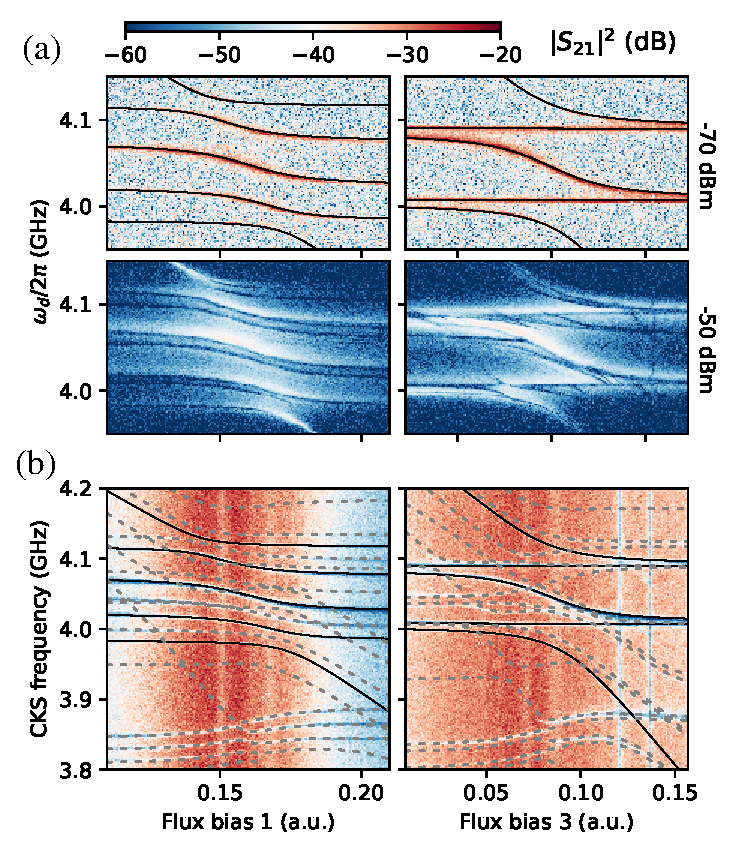
\includegraphics[width=1\linewidth]{Pictures/fig2}
	
	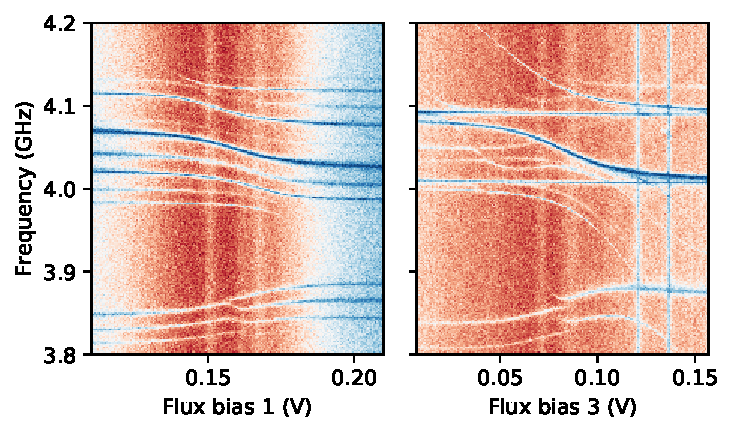
\includegraphics[width=1\linewidth]{Pictures/cktt}
	\caption{\textbf{(a)} Transmission through the chain is observed in five sharp peaks which are shown in dependence on the flux bias voltages 1 (left) and 3 (right) swept around the degeneracy point. In the top row, we show the fit (black lines) of the lowest five transitions of \autoref{eq:bose-hubbard} for $J/2\pi = 41$ MHz, $\omega_i/2\pi \approx 4.05$ GHz ($\Omega = 0$), coinciding with the classical normal modes solution. From top to bottom, as the microwave power is increased (see output power of the VNA on the right), we observe how the system transitions from the classical linear regime to the quantum regime of photon blockade. \textbf{(b)} Cross-Kerr spectroscopy via the the third mode showing the emergent band structure of the system. Dashed lines are fits of the purely quantum transitions with \autoref{eq:bose-hubbard}.}
	\label{fig:transmission}
\end{figure}



To study these purely quantum spectral features in greater detail, we have performed the cross-Kerr spectroscopy on the system, see \autoref{fig:transmission}~(b). Note that we have used the same two configurations of the transmon frequencies as in \autoref{fig:transmission}~(a). Since the additional spectral lines are caused by two-photon processes involving one photon from the VNA (having the frequency of the third mode), and another from the microwave source, their observed frequencies should be corrected by adding the third mode frequency for each bias voltage. However, even without this correction, the emergent band structure is obvious from \autoref{fig:transmission}~(b): the single-excitation band is composed of the classical normal mode frequencies, while quantum two-excitation bands with singly- and doubly-populated sites are located around 4.05 GHz and 3.85 GHz, respectively. The Bose-Hubbard eigenstates with doubly-populated sites have lower energy due to the negative anharmonicity (extracted values of $U/2\pi$ are approximately [-188, -178, -178, -178, -188] MHz), so it is expected that they lie lower in frequency than the states with singly-excited transmons. 


\section{Classical to quantum transition}



\begin{figure*}[t]
	\centering
	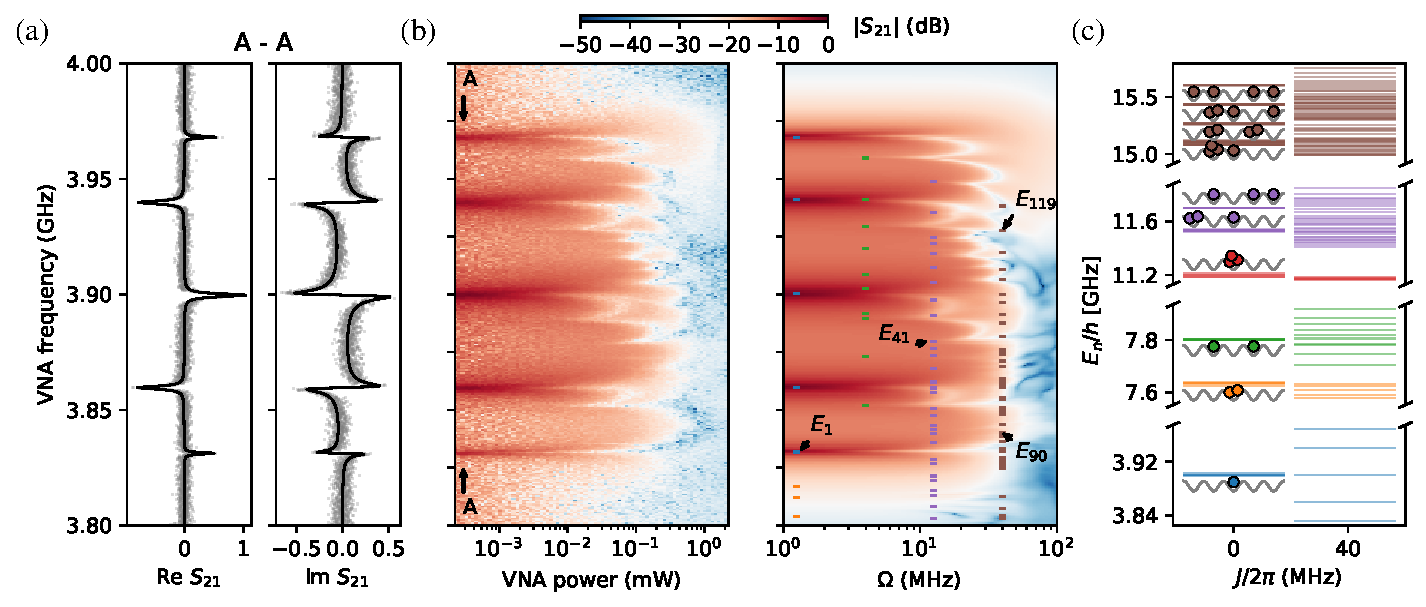
\includegraphics[width=\linewidth]{Pictures/fig3}
	\caption{\textbf{(a)} The analytical solution for the $S_{21}$ in the linear regime (smooth curves) fitted to the low power data (clouds), normalized. \textbf{(b)} Experimental and simulated $S_{21}$. The driving power is calibrated to match the corresponding Rabi frequency of the simulation. The observed structure of the multiphoton peaks is reproduced accurately by the numerical model. \textbf{(c)} The energy level structure of the model with and without interaction (model parameters extracted from fits to the data). We take up to three excitations per site, and up to four excitations total. As shown in panel (b) with dashes, these levels are observable in the experiment and are participating in up to four-photon processes.}
	\label{fig:cq_transition}
\end{figure*}



\begin{figure*}[t]
	\centering
	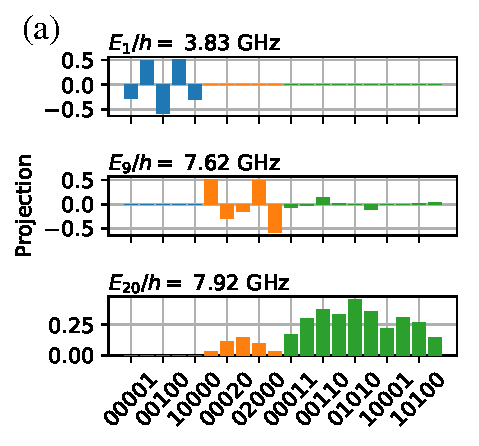
\includegraphics[width=.33\linewidth]{Pictures/eigenstates1}
	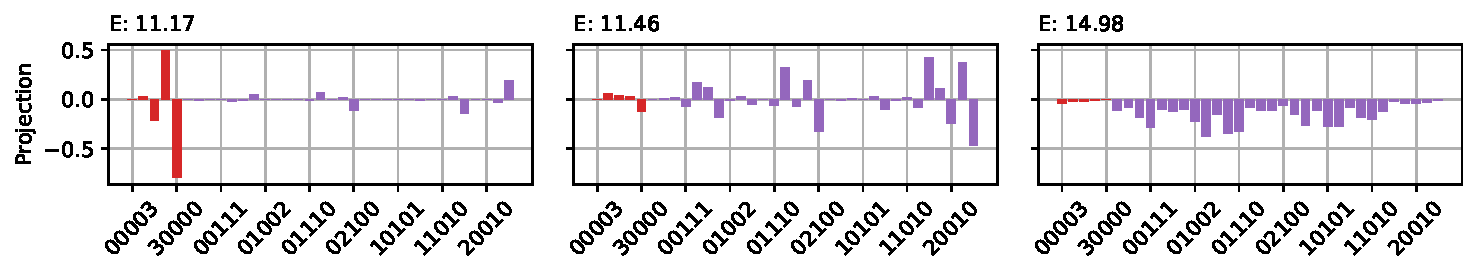
\includegraphics[width=.33\linewidth]{Pictures/eigenstates2}
	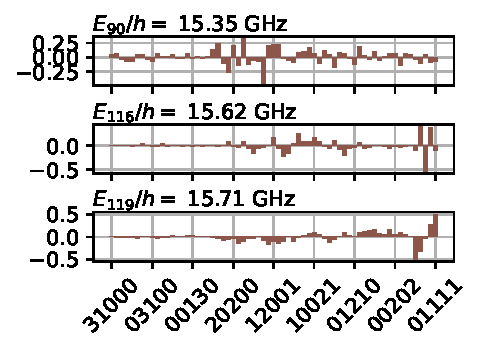
\includegraphics[width=.33\linewidth]{Pictures/eigenstates3}
	\caption{The eigenstates of the system projected onto the unperturbed basis. Colors are the same as in \autoref{fig:cq_transition}~(c). An obvious increase of randomness can be seen as the energy grows. Only the first five excited eigenstates have structure and symmetry (in blue the lowest one is shown) as they obey the correspondence principle. In contrast, no symmetries or even any kind of structure can be found in the distributions found from the higher eigenstates.}
	\label{fig:eigenstates}
\end{figure*}

To further study the energy structure and the non-equilibrium dynamics of the system while it transitions from the classical to quantum regime, we use a direct transmission experiment with fixed degenerate configuration of the transmons, $\omega_i/2\pi = 3.9$ GHz. In the linear regime, we estimate the coupling to the transmission lines and internal dissipations from the fit of the complex transmission coefficient predicted by the linear model which is shown in \autoref{fig:cq_transition}~(a). Using these data, we also estimate the overall attenuation in the measurement system and extract only the transmission through the attenuation and amplification chain. We find that the third mode has nearly unity transmission. This is expected, as from \autoref{fig:transmission}~(a) it is only coupled to a single ``bulk'' transmon, and thus has the least internal dissipation. Since in our full linear model it is impossible to include the pure dephasing separately from the internal dissipation, the relaxation rates from the fit are somewhat larger than true values: we estimate $\gamma_i$ to be [19.9, 1.18, 0.60, 0.95, 18.4] $\mu\text{s}^{-1}$. While the edge ones are probably very accurate, the values for the three internal transmons are determined only approximately. A more subtle method is required to measure the relaxation and pure dephasing rates for them: one obvious way would be to measure them using dispersive readout while all other transmons are far detuned. Also, with the fit we can estimate the disorder in the system; we find $\omega_i/2\pi$ to be [3.878, 3.897, 3.899, 3.902, 3.921] GHz. The disorder from the fit with the linear solution is larger than the disorder expected from the fit in \autoref{fig:transmission}~(a),(b) but still much less than $J$. It is quite possible that the fitted values from the 1D scan are of lower accuracy since the algorithm has to determine 13 parameters from just two curves.

Having the transmons in the degeneracy point, we increase the power of the incident radiation and observe how the spectral lines change their shape and how the multiphoton transitions to the higher energy bands start to appear. The experimental data agrees very well with the numerical steady-state simulation of the five three-level transmons, as can be seen in \autoref{fig:cq_transition}~(b). To achieve visual agreement between the data (where there is enough signal) and the simulation, one should include at least 120 lowest energy states in the model.  Even though the selection rules of the system do not allow us to see all possible multiphoton transitions, we can clearly discern the increase of the density of states and their randomness with increasing band number. At high driving power, the repulsion of energy levels of transmon system gives rise to quasi-chaotic behavior of dips in frequency dependence of transmission amplitude. The frequencies of transitions up to four-photon are shown with colored dashes, which can be identified with the energy bands shown in \autoref{fig:cq_transition}~(c) calculated using the fitted parameters of the model. These effects were also predicted theoretically before \cite{Biella2015} and may be used to prepare various mixtures of many-body states.

Besides the multiphoton transitions which appear as new resonances in the spectrum of the system, the non-classical behavior of the device reveals itself also in the peculiar evolution of the shapes of the classical normal mode resonances. As the driving become stronger, the Autler-Townes splitting occurs leading to dips at these frequencies. In addition, at relatively large driving, multiphoton effects also suppress transmission amplitude at characteristic frequencies related to such processes. The further increase the driving power results in effective shifts of these frequencies due to ``dressing'' of transmon states by incident light. This effect is in fact nothing more than the photon blockade studied extensively in the domain of single-atom lasers \cite{birnbaum2005photon} and predicted for a similar system before \cite{Biella2015}.

To get a deeper insight into the nature of the irregular behaviour of the energy bands shown in \autoref{fig:cq_transition}~(c), we plot in \autoref{fig:eigenstates} several examples of the eigenstates with different energies shown above the plots. As we decompose them onto the unperturbed basis, we see that only the lowest eigenstates corresponding to the classical eigenmodes show structure and symmetry. In \autoref{fig:eigenstates}~(a), $E_1$, we plot of them just the lowest one which has even symmetry and the lowest value of the effective crystal wavelength. Note that the solution of the stationary Shrödinger equation for the lowest modes is identical to the solution of the secular equation of analytical mechanics, which is a manifestation of the Heisenberg correspondence principle for coupled oscillators. The lowest normal mode has nearest neighbors oscillating in antiphase so that all coupling capacitors become charged. But of course the analogy is not fully accurate, as the basis states in the quantum superpositions are the Fock single-photon states while the classical components of the normal mode would be what is called the coherent states in quantum mechanics. Moreover, if we stay with the analogy between our system and the system of trapped bosons, which are physical particles and not just abstract states of an oscillatory system, the intuitive sense of classical analytical mechanics would completely vanish.

Even worse is the situation for the higher levels. One cannot find anymore any bridge to the classical physics for these states. Moreover, we know that the number of degrees of freedom in our system with certainty brings it into chaos in the classical limit, and such systems are notoriously difficult to calculate semiclassically \cite{wintgen1992semiclassical}. We check that the energy spacings indeed follow the Wigner-Dyson distribution of the GOE 
\cite{bohigas1984characterization, livan2018introduction} with vanishing probability to find level intersections. Unfortunately, due to the small number of sites in the chain, one has to include many high-energy states into the histogram which are not accessible in our experiment. Nevertheless, based on the good agreement between the numerical simulation and the experimental data, there remains little doubt that the used model is inappropriate. 

The high energy states couple stronger to each other due to the growing matrix elements of the interaction Hamiltonian, and the bands existing separately from each other for $J=0$ become smeared out.  In \autoref{fig:eigenstates}~(a), $E_9$ is the lowest state from the doublon band (orange states containing two photons on a single site) and is still relatively isolated from other bands. However, $E_{20}$ which is the highest-lying in the two-photon subspace, contains already a significant contribution from the doublon band. Similar is the situation in \autoref{fig:eigenstates}~(b), where we find an isolated trion band in $E_{21}$ and a large entangled state $E_{55}$ (three-photon band upper edge). Finally, in \autoref{fig:eigenstates}~(c) a notable example is the 85\textsuperscript{th} energy state, which is a massive superposition of uncoupled states containing various photon number states encompassing nearly the full entirety of the four-excitation basis. 

It is obvious that eigenstate coefficients in the uncoupled basis are becoming more and more random as the energy is increased and involve more and more basis states. Of course, the appearance of the histograms may change if the basis vectors are reordered. We choose the ordering of the x-axis so that the basis vectors from the lowest energy bands come leftmost, but the ordering inside the bands is arbitrary. However, one can see, for example, that for the state $E_{20}$ in \autoref{fig:eigenstates}~(a) it is not possible to rearrage the green section so that it would have any kind of symmetry. This effect remains even for $J\ll U$ when orange and green bands will be nearly totally uncoupled; moreover, when this condition is not fullfilled, the coupling between adjacent bands introduces even more disorder in the spectrum. So the randomness in the higher energy eigenstates seems to be genuine, irreducible.


\section{Disorder and localization}


\begin{figure}
	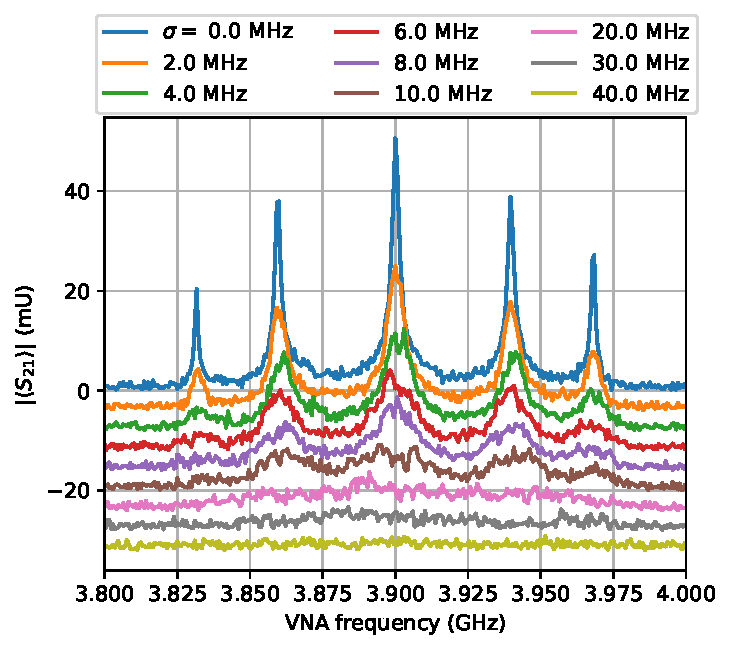
\includegraphics[width=1\linewidth]{Pictures/mbl}
	\caption{Localization and loss of transmission with increasing disorder}
	\label{fig:mbl}
\end{figure}


Since we have good control of the frequencies of the individual qubits, we can can model various strength of disorder in the system. 




\appendix

\section{Linear regime} \label{sec:app_linear}

In the linear regime with no pure dephasing, the Langevin equations for the steady state read:
\begin{equation}
\begin{aligned}
0 &= i(\omega_1 - \omega_d)\hat b_1^\dag - \gamma_1/2 \hat b_1^\dag + i J\hat b_2^\dag + \sqrt{\gamma_1}b_{in}^\dag,\\
0 &= i(\omega_j - \omega_d)\hat b_j^\dag - \gamma_j/2 \hat b_{j}^\dag + i J\hat b_{j-1}^\dag + i J\hat b_{j+1}^\dag,\\
0 &= i(\omega_5 - \omega_d)\hat b_5^\dag - \gamma_5/2 \hat b_5^\dag + i J\hat b_4^\dag,
\end{aligned} 
\end{equation}
with $j = 2,3,4$. The solution of this system shown as the model in \autoref{fig:cq_transition}~(a) is too complex to display; however, for the ideal case it becomes rather simple:
\begin{equation}
\hat b_{{5}}^\dag={\frac {4\,i{J}^{4}\sqrt {\Gamma} \hat b_{in}^\dag}{ \left( i\Delta\,
\Gamma+2\,{\Delta}^{2}-2\,{J}^{2} \right)  \left( i{\Delta}^{2}
\Gamma-2\,i{J}^{2}\Gamma+2\,{\Delta}^{3}-6\,\Delta\,{J}^{2
} \right) }}.
\end{equation}
Here, $\Delta = \omega_d - \omega$. For the case of strong coupling, $J\gg \Gamma$, one can find that the poles of this expression are at $0, \pm J, \pm \sqrt 3 J $. This is a particular case of a more general statement considering the crystal dispersion relation: for a system of size $N$, the crystal momentum takes $N$ values $k = \frac{2 \pi}{N+1} m,\ m=\pm 1, \pm 2... m \leq N/2,\ m\in \mathbb{Z}\  \cup\ {0}$ if $ N $ is odd. Then the corresponding dispersion relation is $E/\hbar = \omega + 2 J \sin k/2$.


\section{Two-qutrit analytical solution}
To make these ideas more transparent we illustrate them using a simple model of a chain of two identical three-level transmons; this case can be solved analytically. However, even for a pair of qutrits the exact analytical expression for the steady state is too cumbersome work with. Therefore we suggest to analyze its series expansion with respect to the driving amplitude. In the leading order in $f$, the density matrix elements in the steady state can be represented as
$$
\rho_{\text{st}} = \rho_{\text{st}}^{ij|i'j'} \propto \sum_{i,j,i',j'} f^{i+j}\, \ket{i,j}\bra{i',j'}
$$
Here $i,\ i'$ correspond to the states of the first transmon and $j,\ j'$ of the second. We split all elements of the density matrix into groups according to its leading order $n$ in $f$. We start from the case $n=1$. In this group there is only single element related to the transmon's ground state, so for this element we have $\rho^{11|11}_{\text{st}}=1$. As the next step, $n=1$, there are four linear equations for density matrix elements $\rho^{11|12}_{\text{st}}$, $\rho^{11|21}_{\text{st}}$, $\rho^{12|11}_{\text{st}}$ and $\rho^{21|11}_{\text{st}}$. Here we take into account the result at the previous step  $\rho^{11|11}_{\text{st}}=1$. We continue this iterative procedure for $n=2, 3, \dots$ and find the remaining density matrix elements. Thus, we finally find the series expansion as

\begin{widetext}
	\begin{align*}
	\langle\sigma_{{\rm st},2} \rangle
	=&\,
	tr  \sigma_{2}  \rho_{\rm st}
	=
	\rho^{11|21}_{\rm st}
	+
	\rho^{22|21}_{\rm st}
	+
	\rho^{33|21}_{\rm st}
	+
	\sqrt{2} \left(
	\rho^{11|32}_{\rm st}
	+
	\rho^{22|21}_{\rm st}
	+
	\rho^{33|21}_{\rm st}
	\right)
	=
	-
	\frac{16 f J}{16 J^2 + (\gamma - 4 i \delta)^2} -
	\\
	- &\,
	\frac{4096 f^3 J^3 (\alpha -i \gamma -4 \delta )}{(2 \alpha -i \gamma \
		-4 \delta ) \left(16 J^2+(\gamma -4 i \delta )^2\right) \left(16 \
		J^2+(\gamma +4 i \delta )^2\right) \left(16 J^2+(\gamma -4 i \delta ) \
		(2 i \alpha +\gamma -4 i \delta )\right)}
	+
	\cdots
	\end{align*}
\end{widetext}
where $\delta = \omega - \varepsilon$ is a detuning. We stress that, in this expansion, each element is calculated in its leading order with respect to $f$. For the sake of simplicity, we consider the case $\gamma \to 0$. In this limit the linear in $f$ term has two poles $\delta = \pm J$ which we attribute to single-photon resonances. The third order term has three additional poles  $\delta = \alpha/2$, $\delta =(\alpha \pm \sqrt{16 J^2 + \alpha^2})/4$ which are attributed to the two-photon process. In fifth order there will be additional three-photonic pole at
$\delta = (\alpha \pm 2J)/3$. The result of the numerical calculation of $\langle\sigma_{{\rm st},2}\rangle$ for different $f$ and $\omega$ is represented in Fig. \ref{fig:2transmon}. As one can see, with the increase of driving power, when driving power become of order of damping, dips appear at frequencies we have determined. This feature is expectable for multi-photonic processes and it is due to effective inverse occupation of the third transmon levels. It occurs when the occupancy of the transmon third level exceeds a second level occupancy, that results in effective suppression of a single-photon process.


There is another approach to find the resonant frequencies responsible for multiphoton processes. Hamiltonian (\ref{H}) in rotating frame does not depend on time explicitly. In addition it conserves excitation number, $N$, so it can be split into independent sectors with particular $N$ which we denote as $H_{(N)}$.
In each sector we find eigenenergies:
\begin{widetext}
$$
\begin{array}{ccc}
H_{(1)} = \begin{pmatrix}
-\delta & J
\\
J & -\delta
\end{pmatrix},
\qquad &
\delta = \pm J;
\\[1em]
H_{(2)} = \begin{pmatrix}
\alpha - 2\delta & \sqrt{2} J & 0
\\
\sqrt{2} J & - 2\delta & \sqrt{2} J
\\
0 & \sqrt{2} J & \alpha - 2 \delta
\end{pmatrix},
\qquad &
\displaystyle
\delta = \frac{\alpha \pm \sqrt{16 J^2 + \alpha^2}}{4}, \quad \delta = \frac{\alpha}{2};
\\[2em]
H_{(3)} = \begin{pmatrix}
\alpha - 3\delta & 2J
\\
2 J & \alpha - 3 \delta
\end{pmatrix},
\qquad & \displaystyle
\delta = \frac{\alpha \pm 2 J}{3};
\\[2em]
H_{(4)} = \begin{pmatrix}
2 \alpha - 4\delta
\end{pmatrix},
\qquad & \displaystyle
\delta = \frac{\alpha}{2}.
\end{array}
$$
\end{widetext}
This result illustrates why there is no specific poles in series expansion of $\langle\sigma_{{\rm st},2}\rangle$ in seventh order: four-photon process is hidden by a two-photon process since both of them have the same energy. This accidental coincidence is a feature of this particular configuration with a couple of three-level systems. For example, if we treat transmons as  four-level systems, then this effect will not occur and four-photon process will be distinguishable.






\bibliography{papers_bibliography}% Produces the bibliography via BibTeX.	
\end{document}